\documentclass[conference]{IEEEtran}
\IEEEoverridecommandlockouts

\usepackage{amsmath,amssymb,amsfonts}
\usepackage{booktabs}
\usepackage{array}
\usepackage{multirow}
\usepackage{graphicx}
\graphicspath{{figures/imported/}{manuscript/figures/imported/}}
\usepackage{cite}
\usepackage{url}
\usepackage{balance}

\newcommand{\BSC}{\ensuremath{\mathrm{BSC}_{6}}}
\newcommand{\R}{\mathbb{R}}
\newcommand{\Ind}{\mathbf{1}}

\title{Spiking Reservoir State-Space Encoding for Perturbation-Characterized Affective EEG Signal Analysis}

\author{
\IEEEauthorblockN{Andrew A. Lane\IEEEauthorrefmark{1}, Wendy Tang\IEEEauthorrefmark{1}, and Brady D. Nelson\IEEEauthorrefmark{2}}
\IEEEauthorblockA{\IEEEauthorrefmark{1}Department of Electrical and Computer Engineering, Stony Brook University, Stony Brook, NY, USA}
\IEEEauthorblockA{\IEEEauthorrefmark{2}Department of Psychology, Stony Brook University, Stony Brook, NY, USA}
}

\begin{document}
\maketitle

\begin{abstract}
Affective electroencephalographic (EEG) event-related potentials (ERPs) are noisy, subject-dependent, and only partially observed projections of neural dynamics, and endpoint accuracy alone does not characterize how a representation behaves under perturbation. We audit four affective-ERP representations spanning a fixed-to-trained spectrum---spectral band-power, ERP-window amplitudes, a fixed (untrained) leaky integrate-and-fire (LIF) reservoir with a six-bin spike-count (\BSC{}) embedding, and a trained EEGNet---under subject-grouped validation and controlled amplitude-noise and channel-dropout perturbations. Accuracy and perturbation-retention dissociate. EEGNet is the most accurate representation (clean balanced accuracy $0.711$) and is almost unaffected by $5$~dB amplitude noise ($99\%$ retention) but loses more under $30\%$ channel dropout ($78\%$); the fixed reservoir is the least accurate ($0.463$) yet shows the highest relative retention ($97$--$99\%$), which an above-chance analysis attributes partly to its proximity to chance; ERP-window features are strongest among the fixed encoders on clean data but the most fragile. Controls---a dimensionality-matched random projection, a label-permutation null, and a single-bin spike-count ablation---bound common confounds. The audit shows that endpoint accuracy and perturbation-retention measure different things, and that high retention can reflect a low operating point rather than useful robustness.
\end{abstract}


\begin{IEEEkeywords}
EEG, event-related potentials, spiking neural networks, reservoir computing, biomedical signal processing, affective computing, perturbation analysis.
\end{IEEEkeywords}

\section{Introduction}
\begin{figure*}[t]
\centering
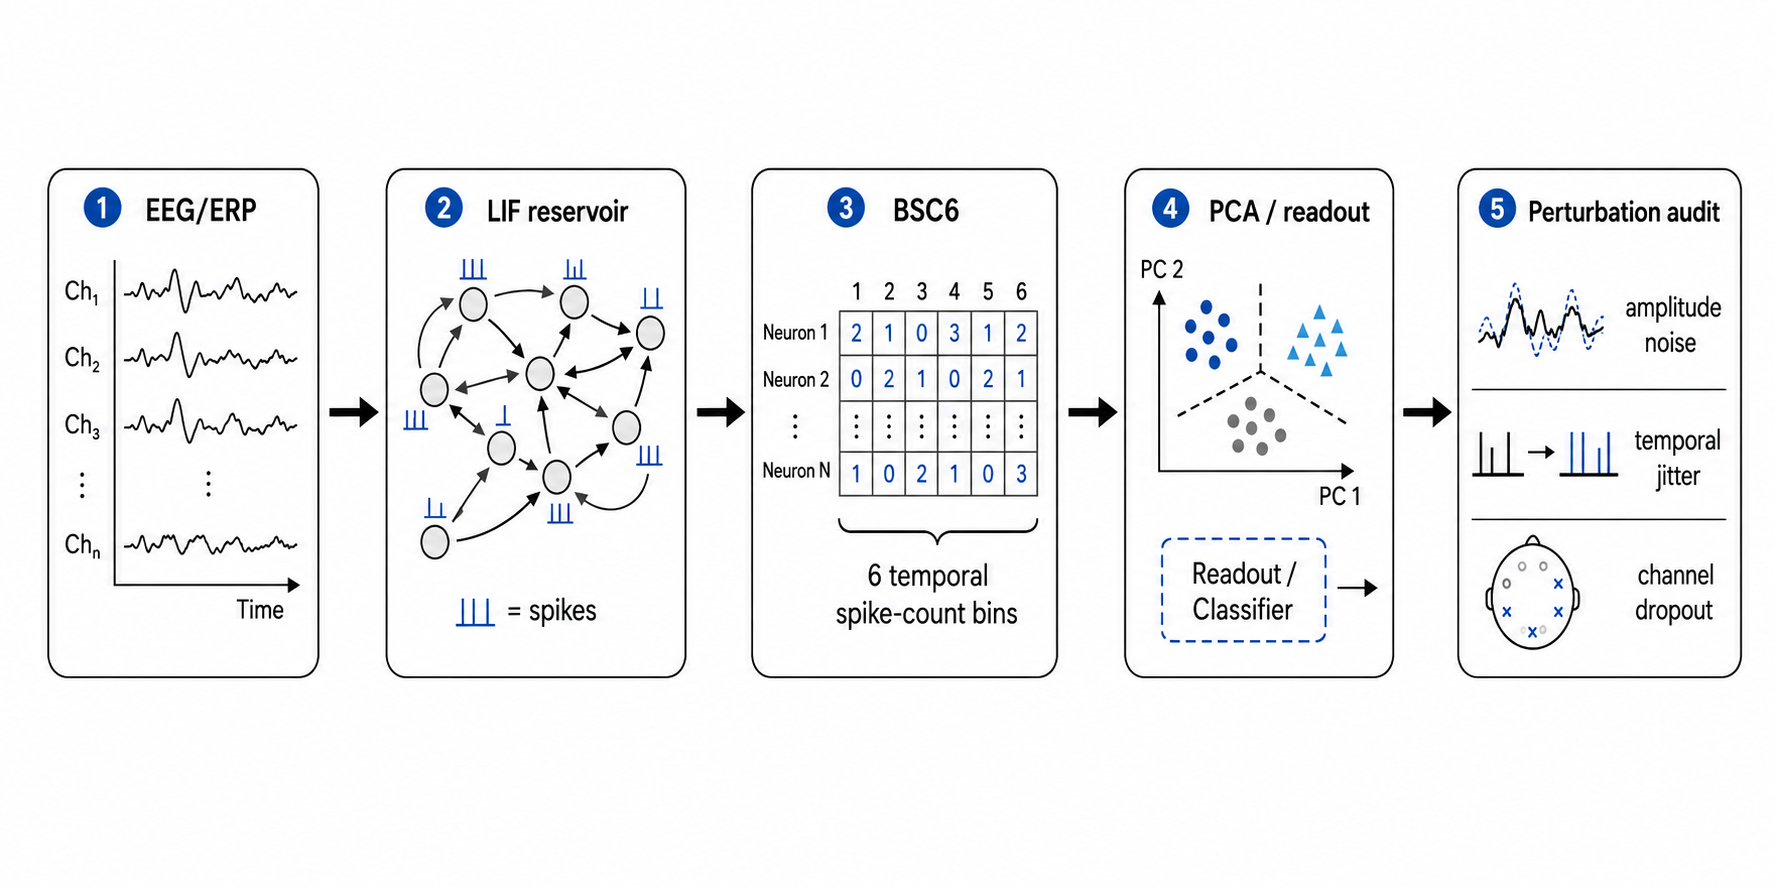
\includegraphics[width=\textwidth]{fig_pipeline_bsc6_audit.png}
\caption{Reservoir encoding and perturbation-audit pipeline. Trial-averaged affective EEG/ERP observations are mapped through a fixed LIF reservoir, summarized by six temporal spike-count bins (\BSC{}), compressed for linear readout, and evaluated under amplitude noise, temporal jitter, and channel-dropout perturbations.}
\label{fig:pipeline}
\end{figure*}

Electroencephalographic event-related potentials (ERPs) are time-locked measurements of neural response dynamics that offer millisecond-scale temporal information for biomedical data analysis, yet the observed waveform is a noisy, low-dimensional, and subject-dependent projection of an unobserved neural dynamical system \cite{makeig2002dynamic,blankertz2011singletrial}. Inter-subject variability, trial averaging, volume conduction, and measurement noise can cause endpoint classifiers to conflate genuine temporal structure with subject-specific nuisance variation, so a representation that performs well on one clean split may not preserve the same signal properties when amplitude noise, temporal misalignment, or channel loss is introduced.

Reporting only endpoint accuracy does not reveal \emph{which} temporal features a representation preserves or suppresses. This gap is acute for spiking encodings: fixed recurrent reservoirs and spiking networks are expressive nonlinear temporal expansions \cite{maass2002real,lukosevicius2009reservoir}, but in EEG/ERP work they are most often evaluated as end-to-end classifiers \cite{gong2023sglnet,craik2019deep} rather than characterized as temporal operators whose discrete spike-count observables remain traceable to post-stimulus time windows.

The perturbation behavior of affective-ERP reservoir encodings---their response to amplitude noise, temporal jitter, and channel dropout---is rarely reported, even though preprocessing and acquisition choices materially affect EEG representations \cite{delpup2025preprocessing,chiang2023depression,guo2025mma}.

This paper audits affective-ERP representations as temporal encoding operators, comparing their perturbation-response profiles rather than only their endpoint accuracy (Fig.~\ref{fig:pipeline}). The representations span a fixed-to-trained spectrum: spectral band-power, ERP-window amplitudes, a fixed (untrained) leaky integrate-and-fire (LIF) reservoir summarized by six post-onset spike-count bins (\BSC{}) and compressed for a linear readout, and a trained EEGNet. The paper isolates the reservoir temporal-encoding component as its focal fixed operator; graph topology, structure--function coupling, and closed-loop analyses belong to other parts of a broader doctoral framework and are outside this submission. The contributions are:
\begin{enumerate}
    \item A perturbation-response audit of affective-ERP representations spanning fixed and trained encoders, under subject-grouped validation with balanced accuracy, macro-F1, and macro one-vs-rest AUC, per-fold confidence intervals, and a permutation null (Sec.~\ref{sec:clean}, Tables~\ref{tab:clean}--\ref{tab:repr_perturb}).
    \item The finding that endpoint accuracy and perturbation-retention \emph{dissociate}: a trained EEGNet is the most accurate and amplitude-stable, the fixed reservoir the least accurate yet most retentive, and an above-chance analysis shows that high retention can reflect a low operating point rather than useful robustness (Sec.~\ref{sec:perturb}, Fig.~\ref{fig:perturbation}).
    \item Characterization of the fixed reservoir encoding as a label-free temporal operator (Eq.~\eqref{eq:operator}), with a single-bin spike-count ablation isolating the reservoir expansion from temporal bin granularity (Sec.~\ref{sec:methods}, Sec.~\ref{sec:clean}).
    \item Controls---fold-local PCA, a dimensionality-matched random projection, and a label-permutation null---that bound common confounds (Sec.~\ref{sec:clean}, Table~\ref{tab:pca}).
\end{enumerate}
Clinical labels and affective categories define the external task structure; the representations are the object of study.

\section{Related Work}
ERP and EEG analysis have traditionally relied on time-window amplitudes and latencies, time-domain descriptors such as Hjorth parameters \cite{hjorth1970eeg}, spectral and wavelet summaries \cite{subasi2007eeg}, and linear statistical models \cite{blankertz2011singletrial}. These features are interpretable and correspond to known components such as the P300 and late positive potential, and source-level analyses show that evoked responses carry structured temporal dynamics \cite{makeig2002dynamic}. Fixed handcrafted windows may, however, underrepresent nonlinear temporal interactions and can be sensitive to subject-specific variability.

Reservoir computing offers an alternative in which a high-dimensional recurrent dynamical system transforms an input sequence into a separable state trajectory \cite{maass2002real,jaeger2001echo,jaeger2004harnessing,lukosevicius2009reservoir}. In liquid state machines, recurrent spiking dynamics induce a nonlinear temporal basis on which a simple readout is trained; related spiking models encode information in spike timing and counts \cite{diehl2015unsupervised,roy2019towards}. This separation of fixed dynamics from a trained readout is attractive for biomedical signal analysis because the reservoir can be studied as a measurement operator rather than as a fully optimized black-box classifier.

Spiking and deep networks have been applied to EEG and ERP signals \cite{gong2023sglnet,lawhern2018eegnet,craik2019deep}, but most studies emphasize endpoint accuracy, while preprocessing and acquisition choices that strongly affect EEG representations are often under-examined \cite{delpup2025preprocessing}. For perturbation-sensitive physiological data, accuracy alone is insufficient: a representation should also be assessed through subject-level generalization, controlled corruption, and representation-geometry analysis \cite{kornblith2019similarity}. Prior work in the ARSPI-Net line developed neuromorphic reservoir feature extraction for affective EEG \cite{lane2023arspi,lane2024arspi}; the present paper isolates and audits the spiking temporal-encoding component as a measurement operator.

\section{Methods}
\label{sec:methods}
\subsection{ERP Observation Model}
Let $X_s^{(c)}\in\R^{C\times T}$ denote the trial-averaged ERP observation for subject $s$ and affective condition $c$, with $C$ electrodes (channels) and $T$ temporal samples; observations are stored as $T\times C$ arrays and transposed before encoding. We treat $X_s^{(c)}$ as a noisy observation of an unobserved neural state trajectory:
\begin{equation}\label{eq:obs}
    \xi_{t+1}=f_\theta(\xi_t,u_t)+\eta_t,\qquad
    x_t=H\xi_t+\epsilon_t,
\end{equation}
where $\xi_t$ is the latent neural state, $H$ is a measurement operator induced by scalp observation, and $\epsilon_t$ captures measurement and preprocessing noise. The perturbations below act directly on this observation model (Sec.~\ref{sec:perturb}).

\subsection{Spiking Reservoir Encoding}
For each electrode trace, the signal is passed through a fixed LIF reservoir of $256$ neurons with recurrent weights $W$ scaled to spectral radius $\rho=0.9$ (near the edge of stability), input weights $W_{\mathrm{in}}$, leak parameter $\beta=0.05$, and firing threshold $\vartheta$. A compact discrete-time representation is
\begin{align}
    v_{t+1} &= \beta v_t + W z_t + W_{\mathrm{in}}x_t - \vartheta r_t, \\
    z_{t+1} &= \Ind[v_{t+1}\geq \vartheta],
\end{align}
where $v_t$ is the membrane state, $z_t$ is the binary spike vector, and $r_t$ denotes reset after threshold crossing. The reservoir is fixed during feature extraction; only the downstream readout is trained.

Post-onset activity is summarized by six equal temporal bins over the window $t\in[10,70]$ in sample units, which at $256$~Hz spans approximately $39$--$273$~ms post-stimulus. For reservoir unit $j$ and bin $k$, the binned spike-count code is $b_{j,k}=\sum_{t\in\mathcal{B}_k} z_j(t)$, $k=1,\ldots,6$. Per-electrode spike-bin features are compressed to $64$ principal components and concatenated across the $34$ channels into a trial-level reservoir representation $E_s^{(c)}\in\R^{2176}$. Writing $s_t=z_t\in\{0,1\}^{N}$ for the reservoir spike state, the encoding is a fixed composition of a nonlinear temporal map, spike-count binning, and the unsupervised projection:
\begin{equation}\label{eq:operator}
E=\phi_{\mathrm{PCA}}\!\big([b_1,\dots,b_6]\big)=\Phi(X),
\end{equation}
so that $E=\Phi(X)$ is a fixed, label-free observable of the input. The principal-component projection is estimated once, unsupervised and without affective labels, over the spike-bin vectors pooled across all observations and electrodes; because the basis is fitted on every subject---including those later held out---it is transductive with respect to subject inclusion, and we report it as a fixed representation audit rather than leakage-free preprocessing (bounded by the fold-local control in Sec.~\ref{sec:clean}). As a temporal-structure control, we also form a single-bin code (BSC$_1$, the total post-onset spike count per unit) processed through the identical PCA pipeline. This window is an early, compact interval that excludes the later P300/LPP ranges available to the ERP-window baseline (Sec.~\ref{sec:methods}); the clean-classification comparison is therefore conservative for the reservoir.

Fig.~\ref{fig:reservoir_dynamics} shows the reservoir-derived computational objects for the three affective conditions: the LIF spike raster, the membrane-potential response, and the \BSC{} embedding projected to two principal components.

\begin{figure*}[t]
\centering
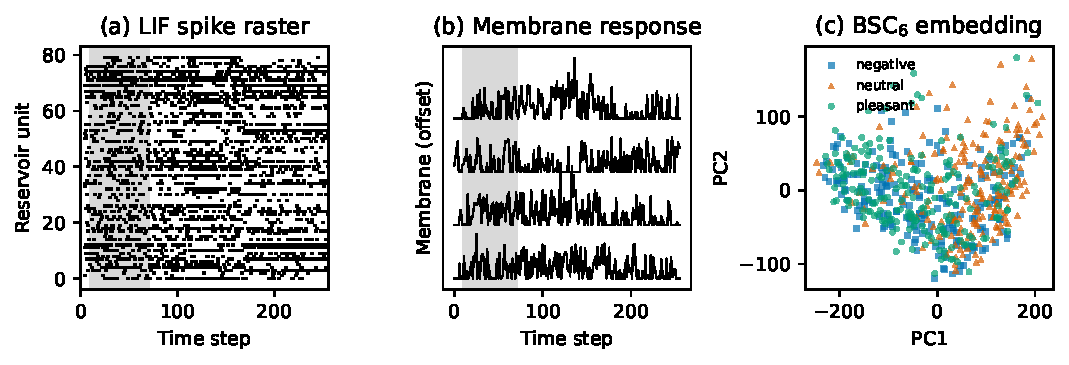
\includegraphics[width=0.92\textwidth]{fig_reservoir_dynamics_inscope.pdf}
\caption{Reservoir-derived computational objects for affective ERP observations. (a)~LIF spike raster for an example trace (shaded region = the $t\in[10,70]$ analysis window). (b)~Membrane response for four units (offset vertically). (c)~\BSC{} embedding projected to the first two principal components, colored by affective condition.}
\label{fig:reservoir_dynamics}
\end{figure*}

\subsection{Baselines and Readout}
Two classical baselines are evaluated under the same subject-grouped protocol. The band-power baseline (A0) uses spectral band-power features ($5$ bands $\times$ $34$ channels $=170$ dimensions). The ERP-window baseline (A0$_e$) uses mean amplitude in three post-stimulus windows---early ($80$--$200$~ms), P300 ($250$--$450$~ms), and late positive potential ($450$--$800$~ms)---per channel ($3 \times 34 = 102$ dimensions). To separate representational robustness from raw dimensionality, we add a dimensionality-matched control: A0 randomly projected to $2176$ dimensions (Gaussian random projection, averaged over five random seeds). The band-power, ERP-window, and reservoir representations use a balanced L2-regularized logistic readout to test separability without a high-capacity classifier.

As a trained deep baseline we evaluate EEGNet-8,2~\cite{lawhern2018eegnet} on the raw $34\times256$ ERP signal under the identical subject-grouped folds, trained per fold (Adam, $80$ epochs) with train-only per-channel standardization. EEGNet ingests the raw signal and has no intermediate feature vector, so its perturbations are applied at the input---comparable to the reservoir's raw-signal recomputation (Sec.~\ref{sec:perturb})---whereas the band-power, ERP-window, and reservoir perturbations are feature-level; the cross-family comparison is therefore approximate.

\subsection{Perturbation Diagnostics}
Two perturbation regimes are separated. Representation-level perturbations corrupt the extracted feature vector; raw-signal recomputation applies perturbations before feature extraction and recomputes the reservoir representation, propagating corruption through reservoir dynamics. Formally, a perturbation $\mathcal{P}_\eta$ acts either on the representation, $E\mapsto\mathcal{P}_\eta(E)$, or on the observation model of Eq.~\eqref{eq:obs}: amplitude noise augments the measurement noise $\epsilon_t$, channel dropout zeroes rows of the measurement operator $H$, and temporal jitter shifts the sampling index of $x_t$. We apply additive amplitude noise (signal-to-noise ratios), temporal jitter of the alignment window, and channel dropout at increasing electrode-removal rates. Performance is balanced accuracy (BA) and macro-F1.

\section{Experimental Protocol}
\subsection{Dataset and Task}
The experiments use a trial-averaged affective ERP dataset with 211 subjects after exclusion of one anomalous subject record. Each subject contributes three affective conditions (negative, neutral, pleasant), yielding 633 subject-condition observations. The ERP traces contain 34 scalp channels downsampled to 256~Hz, with 256 post-stimulus samples per epoch, baseline-corrected relative to onset. Subject-level data are maintained in a restricted research environment; only aggregate, de-identified results are reported. Table~\ref{tab:dataset} summarizes the protocol.

\begin{table}[t]
\caption{Dataset and evaluation protocol summary.}
\label{tab:dataset}
\centering
\small
\begin{tabular}{ll}
\toprule
Item & Value \\
\midrule
Subjects (after exclusion) & 211 \\
Observations & 633 (subject $\times$ condition) \\
Conditions & 3 (neg., neutral, pleasant) \\
Channels / rate / samples & 34 / 256~Hz / 256 \\
Band-power (A0) dim. & 170 ($5{\times}34$) \\
ERP-window (A0$_e$) dim. & 102 ($3{\times}34$) \\
Reservoir embedding ($E$) dim. & 2176 ($64{\times}34$) \\
Validation & subject-grouped 5-fold CV \\
\bottomrule
\end{tabular}
\end{table}

\subsection{Validation}
All results are computed under a single protocol: StratifiedGroupKFold (5 folds, seeds $42$--$46$), train-only standardization, and a balanced L2 logistic readout; observations from the same subject never span train and test. We report means with $95\%$ confidence intervals (CIs) over the 25 folds, and macro one-vs-rest AUC from pooled out-of-fold probabilities. Chance is calibrated by a label-permutation null (100 permutations).

\section{Results}
\subsection{Clean Classification and Controls}
\label{sec:clean}
Table~\ref{tab:clean} reports clean three-class performance. The trained EEGNet is the most accurate representation (BA $0.711$); among the fixed encoders, ERP-window features lead (A0$_e$, $0.616$), above band-power (A0, $0.485$) and the reservoir embedding (A1, $0.463$). A label-permutation null gives BA $0.338\pm0.022$, so every configuration encodes genuine signal (all exceed the null by more than five standard deviations) while the absolute clean separability of the fixed encoders remains modest.

\begin{table}[t]
\caption{Clean subject-level performance (mean $\pm$ 95\% CI over 25 folds). Permutation-null BA $=0.338\pm0.022$.}
\label{tab:clean}
\centering
\small
\setlength{\tabcolsep}{2pt}
\begin{tabular}{llccc}
\toprule
Cfg & Features & BA & F1 & AUC \\
\midrule
D0 & EEGNet (raw, trained) & $0.711\pm0.014$ & $0.710$ & $0.868$ \\
A0$_e$ & ERP-window (102) & $0.616\pm0.016$ & $0.615$ & $0.790$ \\
A0 & Band-power (170) & $0.485\pm0.015$ & $0.483$ & $0.665$ \\
A1 & Reservoir \BSC{} (2176) & $0.463\pm0.013$ & $0.460$ & $0.644$ \\
-- & Reservoir BSC$_1$ (2176) & $0.467\pm0.011$ & $0.465$ & $0.646$ \\
\bottomrule
\end{tabular}
\end{table}

\emph{Temporal-binning ablation.} The single-bin total-count code (BSC$_1$) matches the six-bin code (\BSC{}) on clean classification ($0.467$ vs.\ $0.463$; Table~\ref{tab:clean}) and under perturbation (Sec.~\ref{sec:perturb}). We therefore treat \BSC{} as a temporally localized \emph{audit scaffold} that keeps the observable traceable to post-stimulus windows; the ablation shows that both separability and robustness are driven by the fixed reservoir state-space expansion, not by bin granularity.

\emph{Transduction and component controls.} A fold-local PCA refit (per-fold training subjects) leaves performance unchanged (Table~\ref{tab:pca}); varying the component count over $\{16,32,64,128\}$ keeps BA within $0.461$--$0.491$, so neither the transductive basis nor the $64$-component choice inflates results.

\begin{table}[t]
\caption{Fold-local vs.\ global PCA for the reservoir embedding $E$ (A1). OvR-AUC is macro one-vs-rest from pooled out-of-fold probabilities.}
\label{tab:pca}
\centering
\small
\setlength{\tabcolsep}{3pt}
\begin{tabular}{lccc}
\toprule
PCA basis & BA & Macro-F1 & OvR-AUC \\
\midrule
Global pooled (transductive) & 0.463 & 0.460 & 0.644 \\
Fold-local (per-fold train) & 0.465 & 0.462 & 0.649 \\
\bottomrule
\end{tabular}
\end{table}

\subsection{Perturbation Response and the Accuracy--Retention Dissociation}
\label{sec:perturb}
Table~\ref{tab:repr_perturb} reports perturbation response, and accuracy and retention dissociate. The trained EEGNet remains the most accurate at every level ($0.706$ at $5$~dB, $0.554$ at $30\%$ dropout) and is almost unaffected by amplitude noise ($99\%$ retention), though it loses more under dropout ($78\%$). Among the fixed encoders the retention ordering inverts the clean ordering: ERP-window, strongest on clean data, is the most fragile ($75\%$ and $74\%$), band-power retains $81$--$84\%$, and the reservoir---least accurate on clean data---retains the most ($97$--$99\%$). Across the 25 folds the reservoir's mean absolute BA drop is $0.013$ at $5$~dB and $0.007$ at $30\%$ dropout, versus $0.155$/$0.162$ (ERP-window) and $0.090$/$0.077$ (band-power); using these fold-level drops, its degradation is significantly smaller than either fixed baseline under both perturbations (Wilcoxon signed-rank, $p<0.001$).

High raw retention partly reflects a low operating point. Normalizing by distance to chance, the reservoir's retention falls to $89\%$ (amplitude) and $95\%$ (dropout), while EEGNet---operating far above chance---attains the best amplitude stability ($99\%$) and the reservoir retains the most under dropout. No representation is uniformly best: EEGNet dominates absolute accuracy at every level, the reservoir maximizes relative stability, and retention and accuracy rank the representations differently.

Controls bound common confounds. The dimensionality-matched random projection of A0 (2176-D, five seeds) gives clean BA $0.501\pm0.002$ but collapses to $0.399\pm0.008$ at $5$~dB, tracking A0 ($0.395$) rather than $E$ ($0.449$); channel dropout is channel-matched (all use 34 channels). The single-bin BSC$_1$ embedding is as robust as \BSC{} ($0.452$ at $5$~dB, $0.454$ at $30\%$ dropout), confirming temporal bin granularity plays no role.

\begin{table}[t]
\caption{Perturbation response: balanced accuracy with retention (perturbed$/$clean) in parentheses. A0 random-proj.\ is the dimensionality-matched control (mean over five seeds). EEGNet is perturbed at its raw input (no intermediate feature vector), comparable to Table~\ref{tab:raw_perturb}; the other rows are feature-level.}
\label{tab:repr_perturb}
\centering
\small
\setlength{\tabcolsep}{3pt}
\begin{tabular}{lccc}
\toprule
Representation & Clean & Amp.\ 5 dB & Drop 30\% \\
\midrule
EEGNet (raw, trained) & $0.711$ & $0.706$ (99\%) & $0.554$ (78\%) \\
ERP-window (102) & $0.616$ & $0.461$ (75\%) & $0.454$ (74\%) \\
Band-power A0 (170) & $0.485$ & $0.395$ (81\%) & $0.408$ (84\%) \\
A0 random-proj.\ (2176) & $0.501$ & $0.399$ (80\%) & -- \\
Reservoir $E$ (2176) & $0.463$ & $0.449$ (97\%) & $0.456$ (99\%) \\
\bottomrule
\end{tabular}
\end{table}

\begin{figure}[t]
\centering
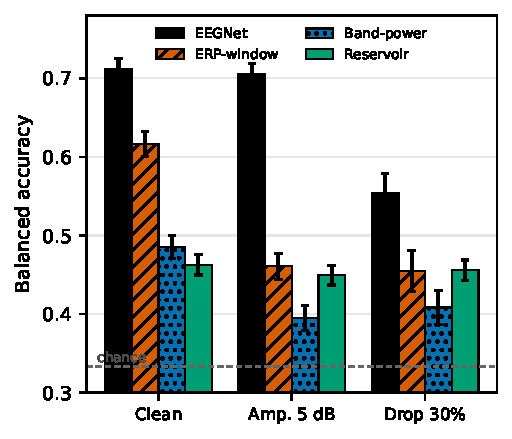
\includegraphics[width=0.92\columnwidth]{ana03_robustness_inscope.pdf}
\caption{Perturbation response across representations. Balanced accuracy (mean, 95\% CI) under clean, $5$~dB amplitude-noise, and $30\%$ channel-dropout conditions. EEGNet is most accurate at every level and most amplitude-stable; among the fixed encoders, ERP-window leads on clean data but degrades most, while the reservoir is least accurate yet most stable---accuracy and retention dissociate. EEGNet is perturbed at its raw input; the others are feature-level. Dashed line = chance.}
\label{fig:perturbation}
\end{figure}

\subsection{Raw-Signal Recomputed Perturbations}
A stricter test corrupts the signal before feature extraction and recomputes the embedding under the same protocol (Table~\ref{tab:raw_perturb}). Clean recomputation reproduces the embedding result ($0.465$). Temporal jitter is the most damaging perturbation ($0.465\!\to\!0.422$), with amplitude noise and channel dropout intermediate ($0.449$, $0.431$); all remain above the permutation null. The embedding is thus reasonably stable even when corruption enters before extraction, but temporal alignment is the dominant sensitivity, consistent with the dependence of the reservoir state trajectory on the input timing.

\begin{table}[t]
\caption{Raw-signal recomputation diagnostics (mean $\pm$ 95\% CI over 25 folds).}
\label{tab:raw_perturb}
\centering
\begin{tabular}{lcc}
\toprule
Condition & BA & Macro-F1 \\
\midrule
Clean recomputation & $0.465\pm0.013$ & $0.462$ \\
Temporal jitter, $\pm 50$ ms & $0.422\pm0.016$ & $0.379$ \\
Amplitude noise, 5 dB & $0.449\pm0.018$ & $0.445$ \\
Channel dropout, 30\% & $0.431\pm0.021$ & $0.402$ \\
\bottomrule
\end{tabular}
\end{table}

\section{Discussion}
The audit supports a bounded, multi-sided reading; no single representation is uniformly best. The trained EEGNet is the most accurate at every condition (clean $0.711$; $0.706$ at $5$~dB; $0.554$ at $30\%$ dropout) and the most amplitude-stable, so a modern deep model, given supervised training, is the performance reference here. Among the fixed encoders evaluated with a linear readout, ERP-window features are strongest on clean data but the most fragile, while the fixed, untrained reservoir is the least accurate yet the most stable in relative terms. Crucially, accuracy and perturbation-retention dissociate: they rank the representations differently, and high retention can reflect a low operating point rather than useful robustness---an above-chance normalization reduces the reservoir's apparent advantage, though it still degrades least under dropout. The reservoir's interest is therefore methodological: it is a fixed, label-free temporal operator whose stability is measurable without any training, not a competitor to a trained classifier. The audit's value is showing that endpoint accuracy alone mischaracterizes how representations behave under controlled corruption. Under raw-signal recomputation (Table~\ref{tab:raw_perturb}) the reservoir embedding remains reasonably stable, with temporal jitter the dominant vulnerability, reflecting its dependence on input timing.

A key negative result delimits the contribution: a single-bin total spike count (BSC$_1$) matches the six-bin code on clean classification and under every perturbation. Temporal bin granularity is therefore not the operative factor; the robustness is a property of the fixed reservoir state-space embedding and its unsupervised compression, not of the temporal binning. The audit framing---characterizing what a fixed encoding preserves under controlled corruption---is what the data support, rather than a claim that temporal structure per se confers an advantage.

Several scope boundaries remain. The dataset is a single affective ERP cohort, and external validation is needed before generalization. EEGNet is perturbed at its raw input while the band-power, ERP-window, and reservoir comparisons are feature-level, so the cross-family perturbation comparison is approximate; a fully matched feature-level deep comparison is left to future work. The study evaluates software-level representations, not neuromorphic hardware energy or latency, which would require measurement on dedicated platforms \cite{davies2018loihi,furber2014spinnaker}. The perturbation diagnostics are controlled tests, not substitutes for full acquisition artifacts, and graph topology and structure--function coupling are not evaluated here.

\section{Conclusion}
We audited four affective-ERP representations spanning fixed and trained encoders under controlled amplitude-noise and channel-dropout perturbations with subject-grouped validation. Endpoint accuracy and perturbation-retention dissociate: a trained EEGNet is the most accurate at every level and the most amplitude-stable, while the fixed, untrained reservoir embedding is the least accurate yet shows the highest relative retention---partly a floor effect, since an above-chance normalization reduces but does not remove its dropout advantage. ERP-window features are strongest among fixed encoders on clean data but the most fragile, and a dimensionality-matched control and a single-bin ablation show the reservoir's stability is neither a dimensionality nor a bin-granularity artifact. The practical message is that high perturbation-retention does not imply useful robustness when absolute accuracy is low, and that characterizing a representation requires reporting both. Future work should extend the audit to multi-cohort data and to deep models perturbed at the feature level for a fully matched comparison.

\textbf{Data Availability and Scope.} The EEG/ERP data used in this study are access-controlled research data and are not redistributed with this submission. Analyses are reported only as aggregate, de-identified results. Clinical labels, where present in the source cohort, are used only to define biomedical signal-analysis context and are not interpreted as diagnostic decisions.

\begin{thebibliography}{99}

\bibitem{maass2002real}
W. Maass, T. Natschl\"ager, and H. Markram, ``Real-time computing without stable states: A new framework for neural computation based on perturbations,'' \emph{Neural Computation}, vol. 14, no. 11, pp. 2531--2560, 2002.

\bibitem{jaeger2001echo}
H. Jaeger, ``The echo state approach to analysing and training recurrent neural networks,'' German National Research Center for Information Technology, GMD Report 148, 2001.

\bibitem{jaeger2004harnessing}
H. Jaeger and H. Haas, ``Harnessing nonlinearity: Predicting chaotic systems and saving energy in wireless communication,'' \emph{Science}, vol. 304, no. 5667, pp. 78--80, 2004.

\bibitem{lukosevicius2009reservoir}
M. Luko\v{s}evi\v{c}ius and H. Jaeger, ``Reservoir computing approaches to recurrent neural network training,'' \emph{Computer Science Review}, vol. 3, no. 3, pp. 127--149, 2009.

\bibitem{diehl2015unsupervised}
P. U. Diehl and M. Cook, ``Unsupervised learning of digit recognition using spike-timing-dependent plasticity,'' \emph{Frontiers in Computational Neuroscience}, vol. 9, p. 99, 2015.

\bibitem{roy2019towards}
K. Roy, A. Jaiswal, and P. Panda, ``Towards spike-based machine intelligence with neuromorphic computing,'' \emph{Nature}, vol. 575, pp. 607--617, 2019.

\bibitem{lane2023arspi}
A. Lane, W. Tang, and B. Nelson, ``Towards ARSPI-Net: Development of an efficient hybrid deep learning framework,'' in \emph{Proc. IEEE Long Island Systems, Applications and Technology Conf. (LISAT)}, Old Westbury, NY, USA, 2023, pp. 1--8.

\bibitem{lane2024arspi}
A. Lane, W. Tang, and B. Nelson, ``Towards ARSPI-Net: Advancing EEG feature extraction with neuromorphic algorithms,'' in \emph{Proc. IEEE Long Island Systems, Applications and Technology Conf. (LISAT)}, Holtsville, NY, USA, 2024, pp. 1--8.

\bibitem{gong2023sglnet}
P. Gong, P. Wang, Y. Zhou, and D. Zhang, ``A spiking neural network with adaptive graph convolution and LSTM for EEG-based brain-computer interfaces,'' \emph{IEEE Trans. Neural Syst. Rehabil. Eng.}, vol. 31, pp. 1440--1450, 2023.

\bibitem{hjorth1970eeg}
B. Hjorth, ``EEG analysis based on time domain properties,'' \emph{Electroencephalography and Clinical Neurophysiology}, vol. 29, no. 3, pp. 306--310, 1970.

\bibitem{subasi2007eeg}
A. Subasi, ``EEG signal classification using wavelet feature extraction and a mixture of expert model,'' \emph{Expert Systems with Applications}, vol. 32, no. 4, pp. 1084--1093, 2007.

\bibitem{makeig2002dynamic}
S. Makeig, M. Westerfield, T.-P. Jung, S. Enghoff, J. Townsend, E. Courchesne, and T. J. Sejnowski, ``Dynamic brain sources of visual evoked responses,'' \emph{Science}, vol. 295, no. 5555, pp. 690--694, 2002.

\bibitem{blankertz2011singletrial}
B. Blankertz, S. Lemm, M. Treder, S. Haufe, and K.-R. M\"uller, ``Single-trial analysis and classification of ERP components---a tutorial,'' \emph{NeuroImage}, vol. 56, no. 2, pp. 814--825, 2011.

\bibitem{lawhern2018eegnet}
V. J. Lawhern, A. J. Solon, N. R. Waytowich, S. M. Gordon, C. P. Hung, and B. J. Lance, ``EEGNet: A compact convolutional neural network for EEG-based brain-computer interfaces,'' \emph{Journal of Neural Engineering}, vol. 15, no. 5, 056013, 2018.

\bibitem{craik2019deep}
A. Craik, Y. He, and J. L. Contreras-Vidal, ``Deep learning for electroencephalogram (EEG) classification tasks: A review,'' \emph{Journal of Neural Engineering}, vol. 16, no. 3, 031001, 2019.

\bibitem{chiang2023depression}
H.-S. Chiang, M.-Y. Chen, and L.-S. Liao, ``Cognitive depression detection cyber-medical system based on EEG analysis and deep learning approaches,'' \emph{IEEE J. Biomed. Health Inform.}, vol. 27, no. 2, pp. 608--616, 2023.

\bibitem{guo2025mma}
Y. Guo, K. Yang, and Y. Wu, ``A multi-modality attention network for driver fatigue detection based on frontal EEG, EDA and PPG signals,'' \emph{IEEE J. Biomed. Health Inform.}, vol. 29, no. 6, pp. 4009--4022, 2025.

\bibitem{delpup2025preprocessing}
F. Del Pup, A. Zanola, L. F. Tshimanga, A. Bertoldo, and M. Atzori, ``The more, the better? Evaluating the role of EEG preprocessing for deep learning applications,'' \emph{IEEE Trans. Neural Syst. Rehabil. Eng.}, vol. 33, pp. 1061--1070, 2025.

\bibitem{kornblith2019similarity}
S. Kornblith, M. Norouzi, H. Lee, and G. Hinton, ``Similarity of neural network representations revisited,'' in \emph{Proc. Int. Conf. Machine Learning}, 2019, pp. 3519--3529.

\bibitem{davies2018loihi}
M. Davies \emph{et al.}, ``Loihi: A neuromorphic manycore processor with on-chip learning,'' \emph{IEEE Micro}, vol. 38, no. 1, pp. 82--99, 2018.

\bibitem{furber2014spinnaker}
S. B. Furber, F. Galluppi, S. Temple, and L. A. Plana, ``The SpiNNaker project,'' \emph{Proceedings of the IEEE}, vol. 102, no. 5, pp. 652--665, 2014.

\end{thebibliography}

\end{document}
